\newpage
\section{Theory and Implementation} \label{sec:theory}

To gain an understanding of the motivations behind this project it is worthwhile to discuss both prior work done with the PDH method, and the motivations behind using it to lock to an atomic source.  The PDH method is often used to lock a laser to an actuated cavity \cite{black1998}.  The Madison group primarily performs laser cooling experiments on Lithium and Rubidium gas.  They need to precisely set laser frequencies at or near key atomic transitions. For example, the Rb87 $5S_{1/2} \rightarrow 5P_{3/2}$ or "D2" transition is the focus of this project.  The closer a laser's frequency is to a desired transition and the smaller the linewidth of that laser, the more efficient any excitation will be.  This has a direct impact on experimental outcome.

\subsection{Brief Overview of Saturated Absorption Spectra}

Using a vapour cell as a frequency selective feature means that the error signal
is being generated from the absorption absorption spectrum of the particular
vapour. To understand what this spectrum looks like, it is sufficient to do a
basic analysis using semi-classical derivations. Because the gas is not
collimated, and is sufficiently hot (room temperature), the constituent
atoms are moving in every direction with the typical Maxwell-Boltzmann speed
distribution. As the primary concern is exposure to a laser beam, the
velocity classes to be considered here are distributed in one direction only,
here referred to as "z":
\begin{gather}
  \rho(v_z) = \sqrt{\frac{m}{2\pi k_B T}} e^{\frac{-m v_z^2}{2k_B T}}
\end{gather}
Each velocity class absorbs the incident beam at a rate that is dependent on
how far it is from a transition resonance. Furthermore, if the atoms are not
stationary, then the incident light is Doppler shifted. This results in the
standard Lorentzian absorption profile with a Doppler correction:
\begin{gather}
  F(\nu, v_z) = \frac{\Gamma / 2 \pi}{(\nu - \nu_0 + \nu_0 v / c)^2 +
  \Gamma^2 / 4}
\end{gather}
where $\nu_0$ is the transition resonance, and $\Gamma$ is the transition
linewidth. Putting these two terms together, and integrating over all velocity
classes in the "z" direction results in a term known as \emph{optical depth}:
\begin{gather}
  \tau(\nu) = \int_{-\infty}^\infty F(\nu, v_z) \rho(v_z) dv_z
\end{gather}
which is a measure of the sample's tendency to absorb an incident photon of
frequency $\nu$. \\

An incident laser beam will enter the vapour cell and be absorbed according to
the optical depth of the medium. However, photons will be re-emitted in a random
direction and so the intensity of the incident beam will be attenuated in the
original propagation direction, depending on its frequency and the quantity
of the medium it has passed through:
\begin{gather}
  I(\nu, z) = I_0 e^{-\tau(\nu)\cdot z}
\end{gather}
Plotting $I/I_0 (\nu, L)$, for some fixed vapour cell length L, and for
values corresponding to the Rb87 D2 transition generates a
a fairly broad absorption spectrum that is essentially Gaussian with a width of approximately 1GHz \cite{maguire2006}.  Using the PDH method to lock to this feature
alone is not atttractive as it generates a very low slope about the null locking
point. If a laser is needed to specifically excite a particular hyperfine
transition, for example, this locking method will not be sufficient. \\

To generate a feature which is suitable for tight locking, a profile known as a
saturated absorption spectrum is generated by exciting the vapour cell with
a beam propagating in the opposite direction of the master laser beam. This beam
is referred to as the "pump" beam, as it serves to pump some of the atomic
population into the excited state and make it innaccesible to the original beam,
hereby referred to as the "probe". The pump beam is normally derived from the
probe beam itself. This results in an additional effect that starves the probe
beam of accessible atoms. For a simple two level system, this can be written as:
\begin{gather}
  S(I_p, \nu, v) = \tau_0 \frac{\nu_0}{c} (P_1 - P_2) =
    \tau_0 \frac{\nu_0}{c} (1 - 2 P_2)
\end{gather}
where $P_1$ and $P_2$ are the ground and excited state population, respectively,
and the other terms are simply normalization constants. An expression for
$P_2$ can be derived that depends on the pump beam intensity, $I_p$, frequency,
$\nu$, here the same as the probe, and the linewidth of the transition
\cite{maguire2006}:
\begin{gather}
  P_2(I_p, \nu, v) = \frac{ (I_p/I_{sat})/2}{1 + (I_p/I_{sat}) +
    4(\nu - \nu_0 - \nu_0 v/c)^2/\Gamma^2}
\end{gather}
Implementing this factor into the prior calculation gives a corrected optical
depth:
\begin{gather}\label{eq:corr_opt_depth}
  \tau'(\nu) = \int_{-\infty}^\infty S(I_p, \nu) F(\nu, v_z) \rho(v_z) dv_z
\end{gather}
The resultant saturated spectrum is shown in \textbf{Figure~\ref{fig:rb87d2abs}}
, for a variety of $I_p$. The emergent feature at the transition resonance is
referred to as a "Doppler-free" feature. This nomenclature refers to the fact
that the velocity class that is most exposed to both the pump and probe beam
is the class around $v_z = 0$. This results in a decrease in probe beam
absorption from that class, and therefore, a higher transmission ratio.
This feature is shown in more detail in \textbf{Figure~\ref{fig:rb87d2abs_closer}}.

\begin{figure}
  \centering
  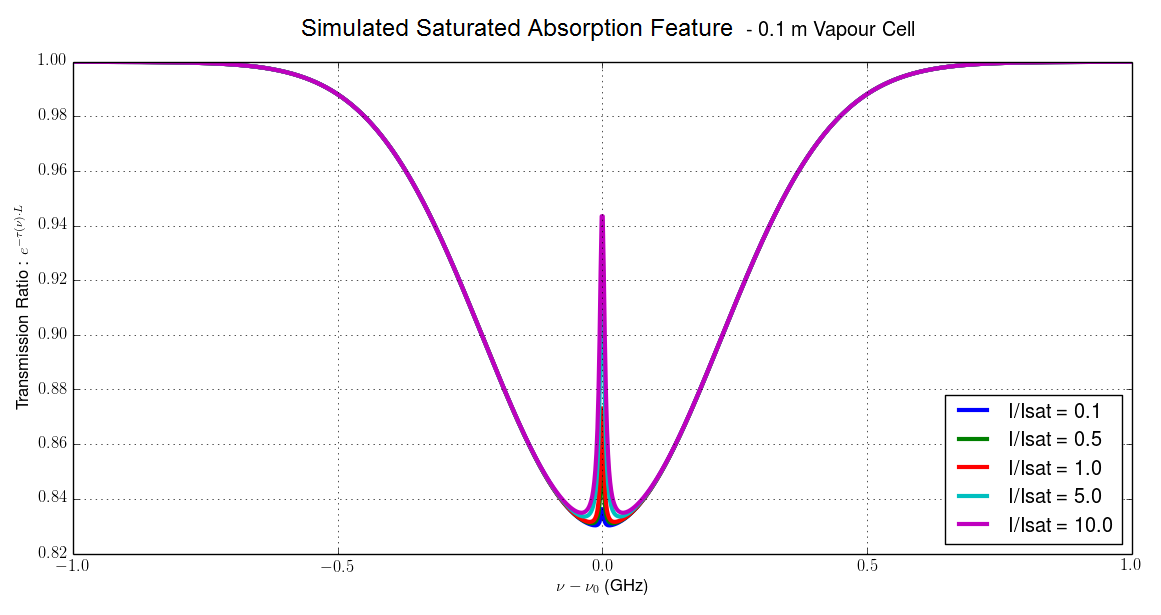
\includegraphics[scale=0.5]{rb_D2_single_absorption.png}
  \caption{Transmission ratio of probe beam through a 0.1m long cell of Rubidium
  gas, near the D2 feature. Optical depth is calculated as shown in
  \textbf{(\ref{eq:corr_opt_depth})},
  and all hyperfine splitting is ignored, (assumed 2-level system) for
  simplicity. The spectrum is plotted for a variety of pump beam intensities
  showing the saturating effect on the velocity classes near $v_z = 0$ at
  resonance.}
  \label{fig:rb87d2abs}
\end{figure}

\begin{figure}
  \centering
  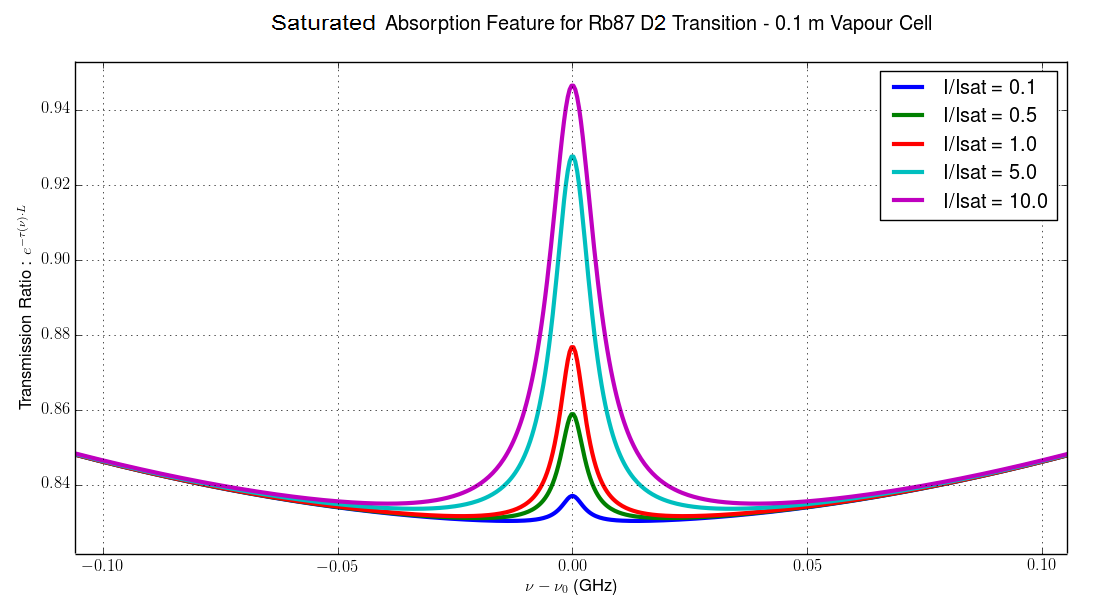
\includegraphics[scale=0.5]{rb_D2_single_absorption_resonance.png}
  \caption{Closer view of \textbf{Figure~\ref{fig:rb87d2abs}}, near the
  resonance.}
  \label{fig:rb87d2abs_closer}
\end{figure}

The model presented here is naive. The Rb87 $5P_{3/2}$ state has 4 hyperfine
levels, and transition from the ground state is goverened by the standard
selection criteria (\cite{steckrb87}, see Figure 2). This produces a much more
complicated absorption feature, with multiple transition and crossover
resonances (\cite{maguire2006}, see Figure 3). Calculating an optimal modulation
frequency for locking about one of the predominant resonance features inside the
Rb87 D2 spectrum can be done with detailed quantum mechanical analysis. It is
unclear if this is necessary, or whether the locking unit should simply be built
with an appropriate phase modulation bandwidth such that heuristic tuning can
attain an optimal result.

\subsection{Optical Phase Modulation}

As it is not possible to process optical signals in the THz range electronically,
it is common to modulate these signals to produce a spectrum about the carrier,
and then down-mix them to RF signals to extract the relevant information.
For optical signals, this is typically done with either an AOM or an EOM. From
a mathematical standpoint, the only difference between the two methods is
what phase modulation depths and frequencies are physically attainable. \\

With AOMs, which use acoustic waves to Doppler shift a beam in the transverse
direction of propagation, there is a distinct tradeoff between modulation
frequency and the resultant power of the outgoing beam.  The AOMs in current use by the Madison Group only have a useful
modulation frequency of approximately 200 kHz \cite{madison14}. \\

The modulation frequency of an EOM is sustainable well into the 100 MHz range,
with modulation depth a function of the driving voltage. Furthermore, as
phase modulation is parallel with the beam propagation, there is no significant
decrease in total beam power as the modulation frequency is increased. High modulation
frequencies do, however, result in higher electrical power consumption.
Typical modulation depths are in the 100mRad range, with a driving voltage of
$\sim 10 V_{pp}$ \cite{thorlabs_eom}. A higher modulation depth demands a higher driving voltage,
which also results in higher power consumption, which may or may not be of
concern. \\

The effect of the phase modulating medium is to induce a phase oscillation
in the incident laser:
\begin{gather}
  E = E_0 e^{i\omega t} \xrightarrow{Phase Modulation}
    E_0 e^{i \omega t + \beta \sin \Omega t}
\end{gather}
where $\beta$ is defined as the modulation depth, in radians, and $\Omega$ is the
modulation frequency. Using the Jacobi-Anger expansion to isolate the sideband
amplitudes,

\begin{gather}
  E_0 e^{i \omega t + \beta \sin \Omega t}  =
  E_0 e^{i\omega t} \sum_{n = -\infty}^{n = \infty} J_n(\beta)e^{in\Omega}
\end{gather}

it is shown that a sideband of frequency $(\omega +n\Omega)$ has amplitude
$J_n(\beta)$, the Bessel function of order $n$, evaluated at $\beta$, the
modulation depth. If the modulation depth is sufficiently small, the following
linear approximation can be made:

\begin{gather}
  E_0 e^{i \omega t + \beta \sin \Omega t}  \approx
    E_0 e^{i\omega t} \left(1 + \frac{\beta}{2}e^{i\Omega t} -
      \frac{\beta}{2} e^{-i\Omega t} \right)
\end{gather}

A visual description of this process is shown in
\textbf{Figure \ref{fig:eom_spectrum}}.
An inspection of Bessel function behaviour near the origin shows that
this approximation quickly becomes invalid for large modulation depths, and
that the carrier amplitude is not conserved. This phenomenon becomes important
when considering the response of a photosensor to the carrier and side-band
amplitudes. These must be tuned such that the signal power is above the noise
floor of the FO receiver, but below the saturation level.

\begin{figure}
  \centering
  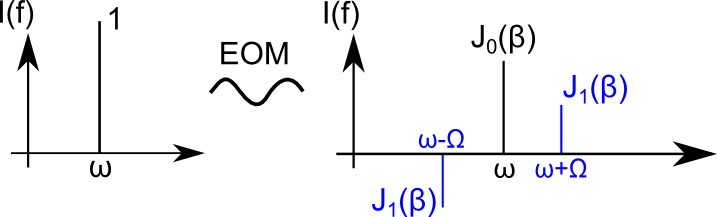
\includegraphics[scale=1.2]{spectrum.pdf}
  \caption{Expected spectrum of beam after phase modulation, to the first
  sidebands. While possibly present and significant, further sidebands can
  be ignored as they will be filtered during mixing.}
  \label{fig:eom_spectrum}
\end{figure}

\subsection{Error Signal Generation}

Obtaining an accurate value for the optimal error signal slope will be a central
development task, if it is not possible to obtain heuristically in
a way that is comfortable for the laboratory staff. Rigorous analysis will
involve some complex quantum mechanical models, but there are precedents for
reference \cite{maguire2006}. \\

The entire PDH error-signal generating setup is depicted in
\textbf{ Figure \ref{fig:setup}}.
The master laser enters at the left, and is immediately split by a
polarizing cube into two beams.  The lower "pump" beam (dashed line), unmodified,
reflects off of several mirrors, and is directed into a chamber full of
Rubidium gas. This beam serves to saturate the absorption ability of the gas,
which results in the a set of Doppler-cancelled features.
The most predominant of these features is used as a locking point. \\

The second "probe" beam is passed into an EOM.  This modulator is fed by a VCO,
running at frequency $\Omega$. As previously discussed, this creates the spectrum
shown in \textbf{Figure \ref{fig:eom_spectrum}}. After being passed through the
vapour cell, the amplitudes of the carrier and the sidebands are attenuated
according to the transmission profile of the saturated absorption feature,
of which a naive representation is shown in
\textbf{Figure \ref{fig:rb87d2abs}}. Let $\hat{F}$ be the operator that
describes the attentuation of the probe beam as it passes through the
vapour cell. Then, the resultant beam is, to the first sidebands:
\begin{gather}
  E_0 e^{i \omega t + \beta \sin \Omega t} \xrightarrow{\hat{F}}
    E_0e^{i \omega t }\left( J_0(\beta)\hat{F}(\omega) +
      J_1(\beta)\hat{F}(\omega + \Omega)e^{i\Omega t} +
        J_1(\beta)\hat{F}(\omega - \Omega)e^{-i\Omega t} \right)
\end{gather}

\begin{figure}
  \centering
  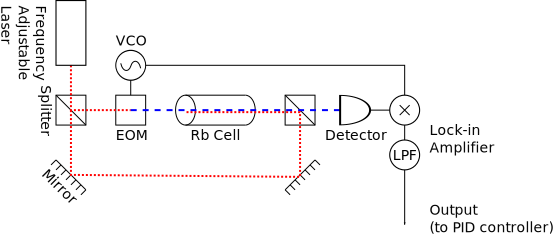
\includegraphics[scale=0.95]{setup.pdf}
  \caption{High level layout of the proposed PDH servo loop using a Rubidium
   vapour cell as the frequency selective element.}
    \label{fig:setup}
\end{figure}

This beam is then coupled into a high-speed fiber optic receiver, a
photosensor unit with bandwidth up to 12GHz. The current produced by the
biased sensor is proportional to the incident optical power. As
$P = |E|^2$, this creates a signal with some mixed frequency components. After
applying a low pass filter to this signal, with a pole at $\sim 1.5 \Omega$,
the following waveform is extracted:
\begin{gather}
  V_1(t) = A(\hat{F}, \omega, \Omega) E_0^2 +
    E_0^2 (J_0(\beta)J_1(\beta))
    (\hat{F}(\omega + \Omega) - \hat{F}(\omega - \Omega))cos(\Omega t)
\end{gather}

Where  $A(\hat{F}, \omega, \Omega)$ is some down-mixed DC term that is dependent
on carrier and side-band powers, as well as the frequency selective element
(it will be filtered out shortly). It is clear even at this stage, that being
able to isolate $(\hat{F}(\omega + \Omega) - \hat{F}(\omega - \Omega))$ will
provide some variable accuracy estimation of the \emph{derivative} of the
saturated absorption spectrum, and will provide a convenient null locking point
at any absorption peaks, which are located at important resonances. To extract
this value explicitly, $V_1$ is mixed with a phase delayed version of the
VCO signal, of frequency $\Omega$ and filtered to extract the DC error signal,
which is explicitly:
\begin{gather}\label{eq:err_sig}
  \epsilon = \alpha E_0^2 (J_0(\beta)J_1(\beta))
    (\hat{F}(\omega + \Omega) - \hat{F}(\omega - \Omega))\cos\phi
\end{gather}
where $\alpha$ is some attentuation factor, dependent on electrical components,
and $\phi$ is the phase delay between the oscillator signal being mixed
and the oscillator signal driving the EOM (same source, one passes through
extra cabling and other components such as buffers, etc). It is clear that
care must be taken to select an appropriate $\phi$ so as to generate a
clear, useable error signal. $\epsilon$ is then fed back into the
laser controller and used to sweep $\omega$ as necessary.
An example error signal, using the naive Rb87 D2 profile in
\textbf{Figure \ref{fig:rb87d2abs}} and generated with different phase modulation
frequencies to show the change in slope about the lock point is shown in
\textbf{Figure \ref{fig:err_gen}\subref*{fig:error_far}}, with an explicit
change in the slope made clear in
\textbf{Figure  \ref{fig:err_gen}\subref*{fig:error_close}}. It is clear from
this analysis that, for this particular absorption profile,
there exists some $\Omega$ between 100kHz and 10MHz that produces
the maximum error signal slope. Maximizing the slope is important as it provides
the smallest drift in frequency for a given change in signal voltage, which
allows any locking system to lock closer to the resonance, given a particular
voltage resolution. If the absorption spectrum for the Rb87 D2 transition has
similar feature size, then it is clear that the existing AOM solution is,
at best, suboptimal.

\begin{figure}
  \begin{tabularx}{\linewidth}{c}
    \subfloat[View far from the null lock point, showing the entire
    feature and generated error signals.]
    {
      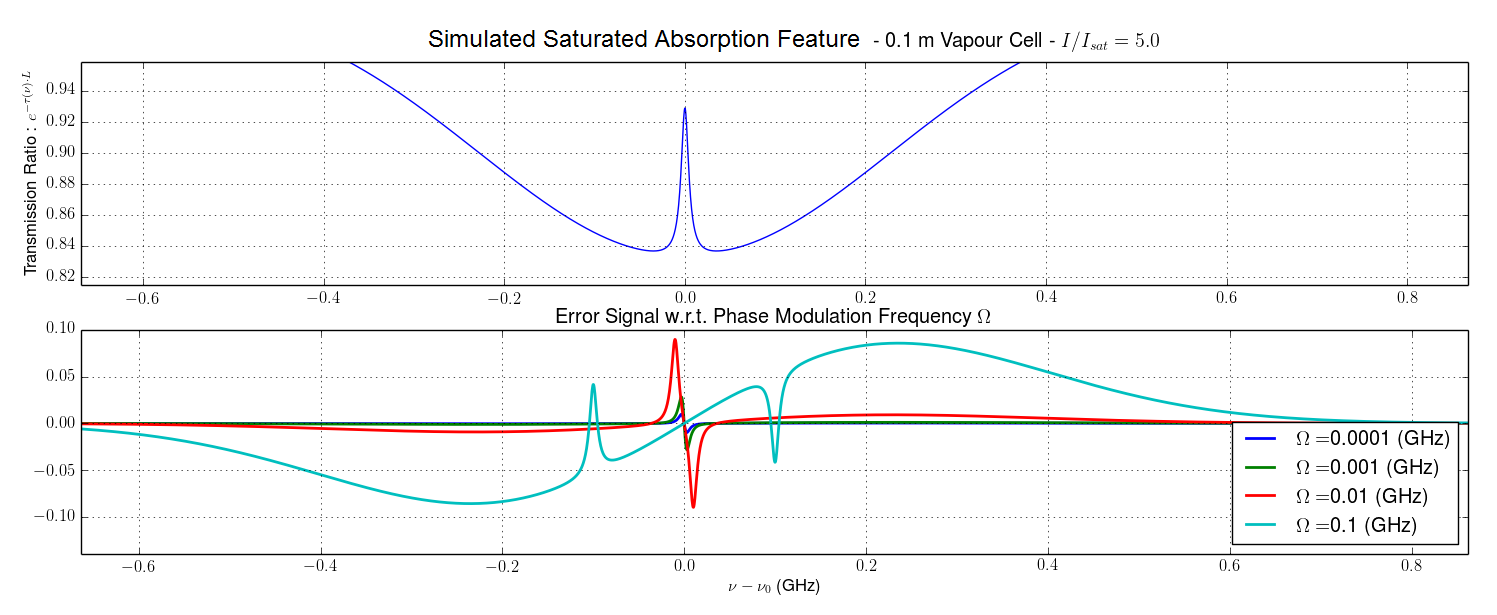
\includegraphics[height=0.5\linewidth, width=\linewidth]
        {rb_D2_error_faraway.png}
      \label{fig:error_far}
    } \\
    \subfloat[View close to the  null lock point, showing the change in
    slope about it as $\Omega$ is varied.]
    {
      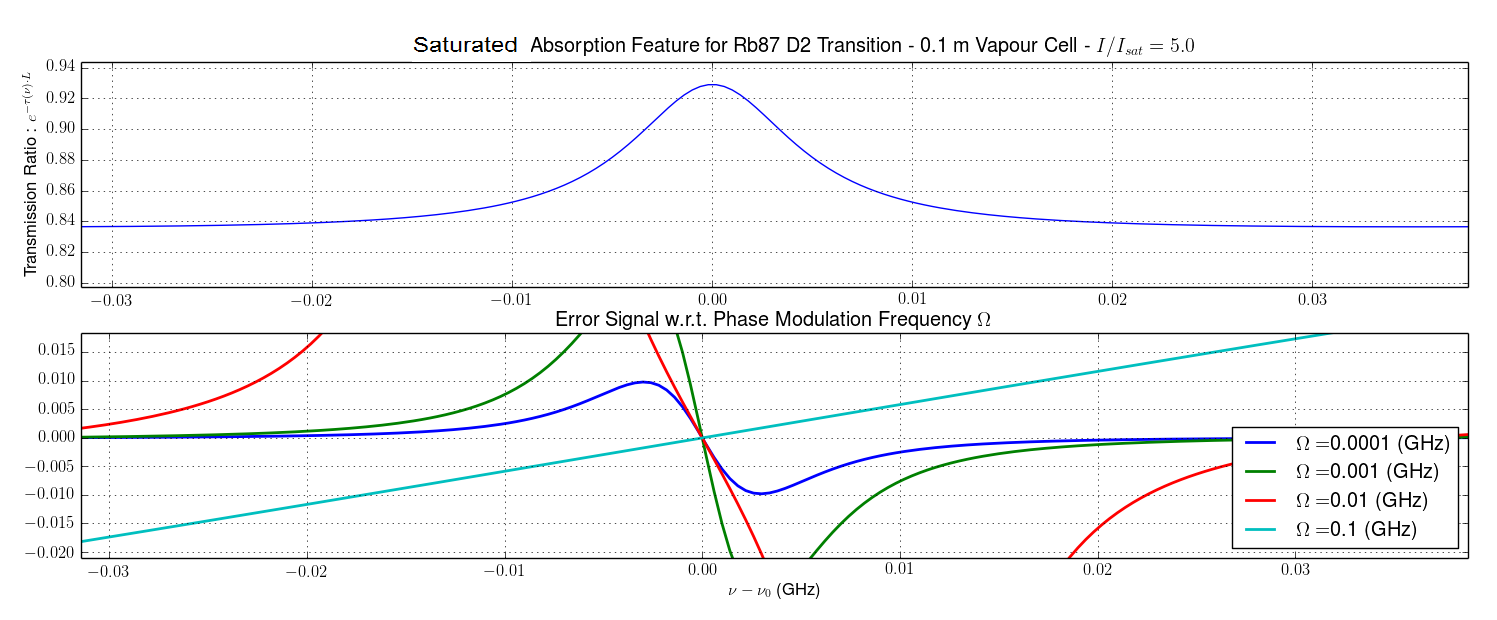
\includegraphics[height=0.5\linewidth, width=\linewidth]
        {rb_D2_error_closer.png}
      \label{fig:error_close}
    }
  \end{tabularx}
  \caption{Generation of an error signal with varying modulation frequencies
    / sideband separation $\Omega$, using (\ref{eq:err_sig}), for a
    saturated absorption feature generated with (\ref{eq:corr_opt_depth}).
    It is clear,
    especially in \protect\subref{fig:error_close}, that there is some
    optimal value for $\Omega$ that creates the largest slope about the
    null lock point. This value will be highly dependent on the size
    of locking features in the saturated absorption spectrum. }
  \label{fig:err_gen}
\end{figure}
